\chapter{Related Work} 
\label{ch:relatedwork}

%This chapter should include a broad and detailed review of relevant existing work. The literature review should provide background and context for the thesis work. The subsections may be organized in whatever
%manner seems best suited to the material---chronological, or by topic, or
%according to some other criteria (e.g., primary versus secondary resources).

Algfoor et al. \cite{abd2015comprehensive} provide an overview of pathfinding algorithms and how they convert real three-dimensional spaces into machine-traversable spaces. The representations of the environment that each algorithm takes can vary, from 2D or 3D grids to graphs or maps. Some algorithms use a waypoint system by which the robot breaks down its path into separate chunks based on pre-determined locations. There are also hierarchical approaches such as probabilistic roadmaps and random tree traversal. The most prevalent graph representation model for robotics pathfinding algorithms is a 2D square grid, and some of the algorithms that use these graphs are the Exhaustive and Monte-Carlo Iterative Taxing Algorithms and the Jump Point Search Algorithm. The Monte-Carlo algorithm relies on multiple calculation agents that randomly alternate once they reach an obstacle. An example of what one of these two-dimensional grids is provided by Jiang et al.\cite{jiang2018eight} in Figure \ref{fig:Environment}.
\begin{figure}[H]
    \centering
    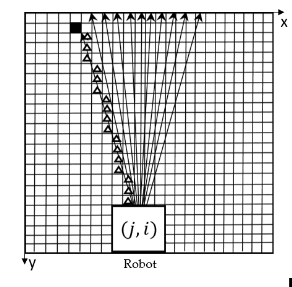
\includegraphics{images/EnvironmentRepresentation.PNG}
    \caption{Example environment representation}
    \label{fig:Environment}
\end{figure}
\section{Algorithm examples}
Bnaya et al. \cite{bnaya2013multi} present the Monte-Carlo Iterative Taxing Algorithm, which utilizes a few different software agents to traverse a 2-Dimensional grid. These software agents each can recognize when they would collide with either another agent or an obstacle, and they then must pay a “tax” in the form of waiting for an amount of time. By keeping track of all of these collisions, the algorithm constructs a series of "penalty tables" that store and compare the amount of tax paid per path found by the algorithm. The best path chosen by this algorithm will be the one with the lowest average sum of the penalty tables associated with the traversal.
\par
Karur et al. \cite{karur2021survey} discuss various extensions of the A* pathfinding algorithm, and therefore this resource can be used to great effect when implementing another version of the A* algorithm. The types of the A* algorithm discussed in this survey are shown in Table \ref{tab:algvariations}.
\begin{table}[H]\centering\footnotesize
    \caption{Variations of the A* algorithm presented by Karur et al.}\label{tab:algvariations}
    \begin{tabular}{|c|}
        \hline
        \textbf{A* Algorithm Variations} \\ \hline
        A* \\ \hline
        Hierarchical A* \\ \hline
        Hybrid A* \\ \hline
        Guided Hybrid A* \\ \hline
        A* with equal step sampling \\ \hline
        Diagonal A* \\ \hline
        A* with smart heuristics \\ \hline
        Lifelong Planning A* \\ \hline
    \end{tabular}
\end{table}
Using these other variants of the A* algorithm, it is possible to get a more full understanding of what different modifications will do to the basic A* algorithm. When this project makes its own version of the base A* algorithm, this context will be extremely useful in evaluating the effectiveness of the new algorithm.
\par
Vermette \cite{vermette2011survey} also discusses variations on the A* algorithm, which will provide even further context into what modifications can be made to the A* algorithm and how; in a very similar fashion to the Karur source listed previously.
\par
Belwariar's \cite{belwariar_2021} GeeksforGeeks article offers a solution for an implementation of the basic A* algorithm, and therefore can be used as a basis for my own understanding/implementation of the algorithm in this project. This algorithm takes in a grid of binary values (0 or 1) where a 0 means that the coordinate is non-traversable, whereas a 1 means it can be traversed. This type of grid can be used by my version of the A* algorithm, and stored in either a text file or a csv such that it can be easily imported to the simulation tool.
\par
Harabor and Grastien \cite{harabor2011online} designed an algorithm called the jump point search (JPS) algorithm which is an improvement on the A* algorithm. The JPS algorithm assesses all adjacent nodes in a 2D grid that are adjacent to the starting direction for each traversal. The algorithm uses "jump points" to limit the number of potential paths that the traversal needs to consider, therefore drastically reducing the amount of time it takes to arrive at the correct path for the robot/agent to take to its destination. Harabor and Grastien used the environment models proposed by Nathan R. Sturtevant \cite{sturtevant2012benchmarks} when testing their algorithm.
\section{Relevant Equations}
Henkel et al. \cite{henkel2016energy} developed a pathfinding algorithm that factors in the required battery power of each different path when making a decision on which it should take. This type of approach should be useful in informing how this proposed project can add battery power cost as an additional consideration for the autonomous robot, and therefore may be applicable to the A* algorithm that this project also aims to modify. This specific implementation of a pathfinding algorithm uses Djikstra's algorithm and the "Dynamic Window Approach" to simulate and choose from a number of possible trajectories for an autonomous field robot. In the end, the researchers concluded that their algorithm reduced the power consumption of an autonomous robot by almost ten(10) percent.
\par
Their algorithm factors in energy cost when considering routes to take\cite{henkel2016energy}, meaning that a similar approach can be used for calculating the energy required for other pathfinding algorithms. By analyzing the Electrical Energy, Frictional Energy, and Acceleration energy of the robot, it is possible to get an accurate projection by taking all of their sums. The Electrical Energy is calculated by taking the Voltage(U), the Current(I), and the time(t), and multiplying them together in this equation:\begin{equation}
    E_{et} = U\times I\times t
\end{equation}
Similarly, the Frictional Energy can be obtained by multiplying the velocity(v), the frictional coefficient(C), and the distance traveled(s):\begin{equation}
    E_{fric} = v \times C \times s
\end{equation}
And finally the Acceleration Energy can be calculated by multiplying the mass of the robot(m) with the acceleration(a) and the distance it travels(s):\begin{equation}
    E_{acc} = a \times m \times s
\end{equation}
These equations\cite{henkel2016energy} should be general enough to be applied to any robot and any pathfinding algorithm in order to get the energy required for a given path/trajectory.
\par
Li and Wang \cite{li2014coordinated} provide formulas for calculating the energy cost of wheeled robots attempting to climb slopes. In the proposal defense, there was a question raised about including topography in the calculations of energy cost along the ground. The equations presented in Li and Wang's paper, when included in the context of this project's algorithm comparison tool, are able to give a proper approximation of the true energy cost of traversing a slope with a wheeled robot. This approximation is used as a weight for the energy cost of traveling a given distance both in the modified A* algorithm constructed in this project, and in the comparison tool when calculating the energy cost of other algorithms.
\par The equations they use for calculating the traction efficiency of a six-wheeled robot are as follows:
    \begin{equation}
        T = F_{DP} \times l + F_{N} \times e
    \end{equation}
    \begin{equation}
        F_{DP} = \frac{T}{ r_{s}} - F_{N} \times \frac{e}{r_{s}}
    \end{equation}
Where T is 